% Created 2023-08-13 dom 12:52
% Intended LaTeX compiler: pdflatex
\documentclass[11pt]{article}
\usepackage[utf8]{inputenc}
\usepackage[T1]{fontenc}
\usepackage{graphicx}
\usepackage{grffile}
\usepackage{longtable}
\usepackage{wrapfig}
\usepackage{rotating}
\usepackage[normalem]{ulem}
\usepackage{amsmath}
\usepackage{textcomp}
\usepackage{amssymb}
\usepackage{capt-of}
\usepackage{hyperref}
\usepackage{../modern}
\bibliography{../sample.bib}
\usetheme{JuanLesPins}
\usecolortheme{dove}
\setcounter{secnumdepth}{2}
\author{Luis Eduardo Galindo Amaya (1274895) \\
Juan Fransisco Perez Valdez  (324342)}
\date{29 de Junio 2023}
\title{Identificación y manejo de material de laboratorio}
\hypersetup{
 pdfauthor={Luis Eduardo Galindo Amaya (1274895) \\
Juan Fransisco Perez Valdez  (324342)},
 pdftitle={Identificación y manejo de material de laboratorio},
 pdfkeywords={},
 pdfsubject={},
 pdfcreator={Emacs 27.1 (Org mode 9.3)}, 
 pdflang={Spanish}}
\begin{document}

\modentitlepage{../images/escudo-uabc-2022-1-tinta-pos.png}
\tableofcontents
\pagebreak
\datasection{Individual}

\section{Hola}
\label{sec:orgc8db13c}
Nam euismod tellus id erat.  Pellentesque dapibus suscipit ligula.  
Donec posuere augue in quam.  Etiam vel tortor sodales tellus ultricies
commodo.  Suspendisse potenti.  Aenean in sem ac leo mollis blandit.  
Donec neque quam, dignissim in, mollis nec, sagittis eu, wisi.  

\subsection{Ejemplos de codigo desde archivos externos}
\label{sec:org813d8b5}
\texttt{Phasellus lacus}.  Etiam laoreet quam sed arcu.  Phasellus at dui in 
ligula mollis ultricies.  Integer placerat tristique nisl.  Praesent 
augue.  Fusce commodo.  Vestibulum convallis, lorem a tempus semper, 

\lstinputlisting{code/test.el}

\lstinputlisting{code/main.c}

\lstinputlisting{code/makefile}

Using \texttt{biblatex} you can display a bibliography divided into sections, 
depending on citation type. Let's cite! Einstein's journal paper 

\subsection{Nam vestibulum accumsan nisl}
\label{sec:org3460398}
dui dui euismod elit, vitae placerat urna tortor vitae lacus.  Nullam 
libero mauris, consequat quis, varius et, dictum id, arcu.  Mauris 

\section{asdad}
\label{sec:orga224692}
mollis tincidunt felis.  Aliquam feugiat tellus ut neque.  Nulla 
facilisis, risus a rhoncus fermentum, tellus tellus lacinia purus, et 
dictum nunc justo sit amet elit \cite{einstein}. 

\section{Hola como estan kaskas}
\label{sec:org86f2911}
Cum sociis 
natoque penatibus et magnis dis parturient montes, nascetur ridiculus 
mus.  Nulla posuere.  Donec vitae dolor.  Nullam tristique diam non 
turpis.  Cras placerat accumsan nulla.  Nullam rutrum.  Nam vestibulum
accumsan nisl.

\begin{figure}[htbp]
\centering
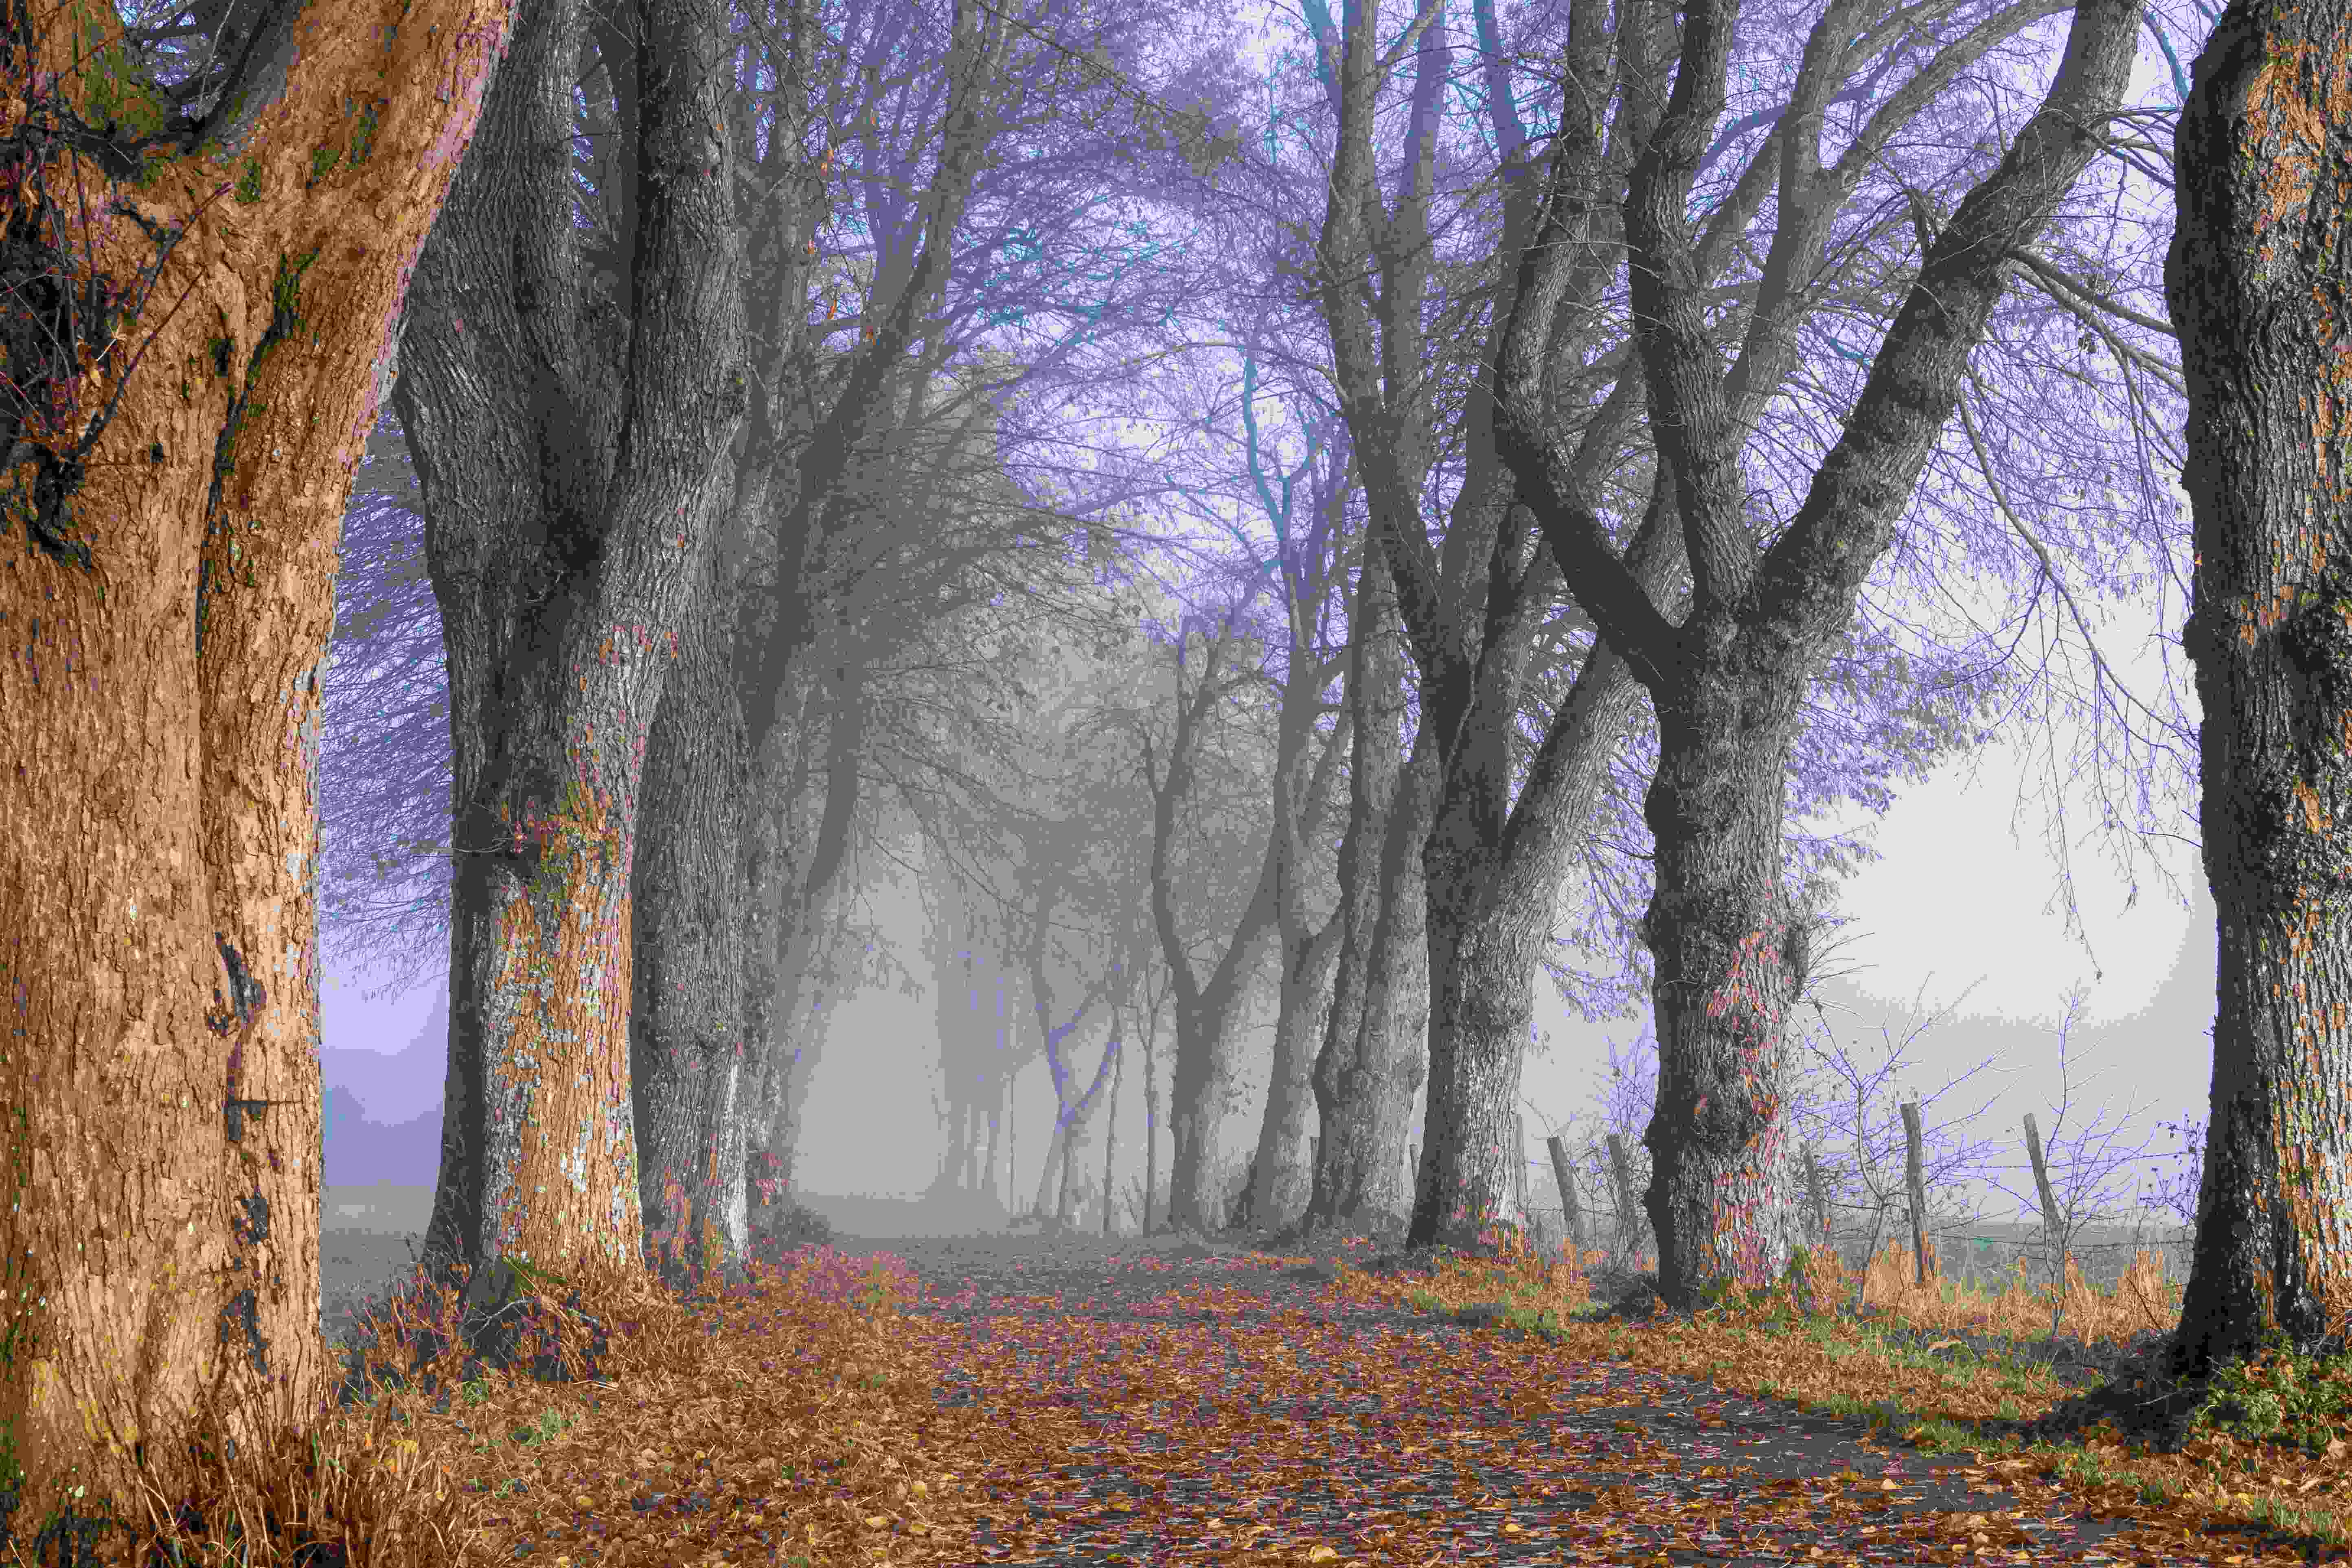
\includegraphics[width=8cm]{images/2019-11-30-Marienallee_Dahlem-7978.jpg}
\caption{Marienallee in Dahlem, Euskirchen district}
\end{figure}

\subsection{Test}
\label{sec:org8eca318}
Lorem ipsum dolor sit amet, consectetuer adipiscing elit.  Donec 
hendrerit tempor tellus.  Donec pretium posuere tellus.  Proin quam 
nisl, tincidunt et, mattis eget, convallis nec, purus.  

\begin{verbatim}
import numpy as np

def incmatrix(genl1,genl2):
    m = len(genl1)
    n = len(genl2)
    M = None #to become the incidence matrix
    VT = np.zeros((n*m,1), int)  #dummy variable

    #compute the bitwise xor matrix
    M1 = bitxormatrix(genl1)
    M2 = np.triu(bitxormatrix(genl2),1) 

    for i in range(m-1):
        for j in range(i+1, m):
            [r,c] = np.where(M2 == M1[i,j])
            for k in range(len(r)):
                VT[(i)*n + r[k]] = 1;
                VT[(i)*n + c[k]] = 1;
                VT[(j)*n + r[k]] = 1;
                VT[(j)*n + c[k]] = 1;

                if M is None:
                    M = np.copy(VT)
                else:
                    M = np.concatenate((M, VT), 1)

                VT = np.zeros((n*m,1), int)

    return M
\end{verbatim}
\captionof{figure}{Hola como esatn}

\section{Test Table}
\label{sec:orgd42b19f}

\begin{table}[htbp]
\centering
\begin{tabular}{|l|l|l|}
\hline
Hola & Como & Estan en este dia\\
\hline
Aliquam posuere. & jk dsadsa & jk eweweq\\
j wqeqwe & k eweqw & jkjkj\\
 &  & \\
 &  & \\
\hline
\end{tabular}
\caption{Hola}

\end{table}

\section{Referencias}
\label{sec:org34be946}
\printbibliography[heading=none]
\end{document}
